%!TEX root = principal.tex
\chapter{Sistema SCADA MANGO}
Mango é uma solução SCADA/HMI open source que roda em um sevidor internet java. Logo toda interface dele é através de um navegador. Muito embora ele seja open source, existem versões aprimoradas dele que apresentam umas facilidades a mais, mas a versão básica já permite fazer um sistema SCADA completo.

\section{Instalação}
Vide \emph{http://infiniteautomation.com/wiki/wiki.php}, a instalação é simplesmente descompactar um arquivo zip e rodar um script para abrir o programa. Basta ter o java 1.7 instalado.

\section{Uso}
Ao rodar o mago, ele abre a tela mostrada na figura \ref{fig:mango_login}. A página do mango pode ser acessada novamente pelo endereço \emph{http://localhost:8080}. O login padrão é \textbf{admin}, senha \textbf{admin}.
\begin{figure}[hbt]
	\begin{center}
		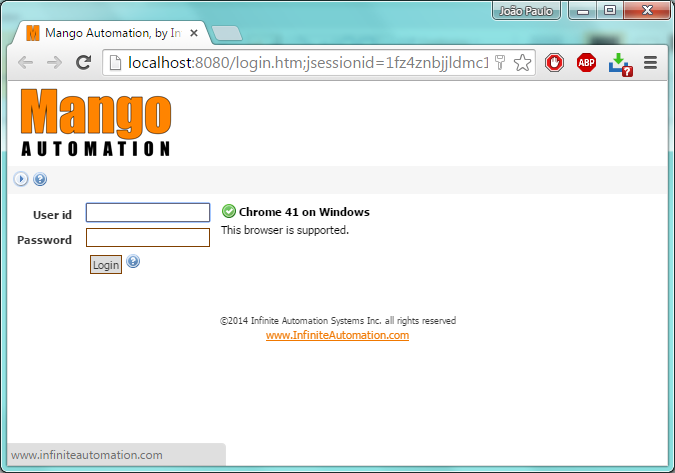
\includegraphics[width=\textwidth]{figuras/mango_login}
	\end{center}
	\caption{Tela de login do mango.}
	\label{fig:mango_login}
\end{figure}

O topo da tela do mango pode ser visto na figura \ref{fig:mango_topo}. Na parte mais superior tem os indicadores de eventos e alarmes, seguido dos links para as diversas áreas do mango.
\begin{figure}[hbt]
	\begin{center}
		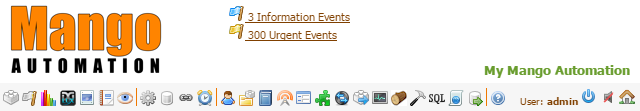
\includegraphics[width=\textwidth]{figuras/mango_topo}
	\end{center}
	\caption{Topo da tela do mango.}
	\label{fig:mango_topo}
\end{figure}

Um dos primeiros pontos a ser definido é o das fontes de dados do sistema. Chega-se nisto clicando no ícone \emph{data sources}, vide figura \ref{fig:mango_sources}. São possíveis diversos tipos diferentes de fontes de dados, mas para nós no momento os que vão interessar são o \textbf{Modbus I/P}, o \textbf{Modbus Serial} e o \textbf{Virtual Data Source}, este último principalmente para simulação.
\begin{figure}[hbt]
	\begin{center}
		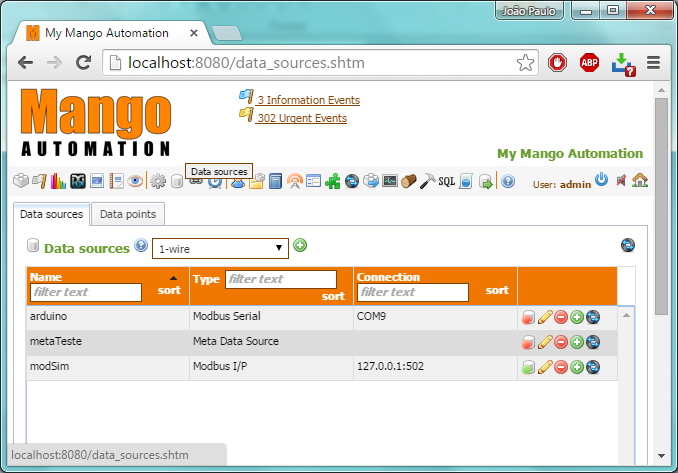
\includegraphics[width=\textwidth]{figuras/mango_sources}
	\end{center}
	\caption{Tela de fontes de dados.}
	\label{fig:mango_sources}
\end{figure}

Para cada fonte de dados, são criados pontos (\emph{data points}), correspondentes a uma tag. No caso de uma fonte virtual, há opções quanto ao tipo de dado (binário, multi-estado, numérico, texto) e quanto ao valor automático, vide figura \ref{fig:mango_virtual}.
\begin{figure}[hbt]
	\begin{center}
		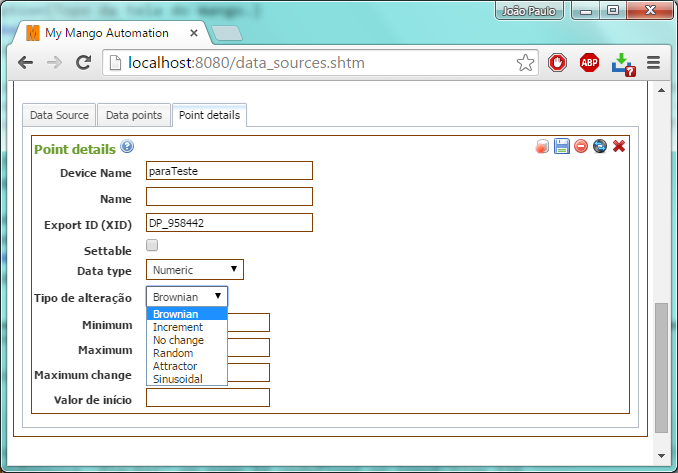
\includegraphics[width=\textwidth]{figuras/mango_virtual}
	\end{center}
	\caption{Definição de dados virtuais para simulação.}
	\label{fig:mango_virtual}
\end{figure}

O protocolo modbus é um dos utilizados na automação industrial. Existe uma implementação do modbus serial para arduino, que é implementado pelo uso da biblioteca \textbf{SimpleModbusSlave}, que faz o arduino trabalhar como um escravo modbus. O data source Modbus Serial nos permite então obter dados de um arduino, seguindo este protocolo.

A configuração do Modbus para a comunicação com o arduino é tal como mostrado na figura \ref{fig:mango_modbus}. É importante que a porta seja a mesma do arduino, bem como bit rate (baud rate), data bits, stop bits, stop bits e parity. O encoding deve ser do tipo RTU e deve se marcar a caixa \textbf{Contiguous batches only}.

\begin{figure}[hbt]
	\begin{center}
		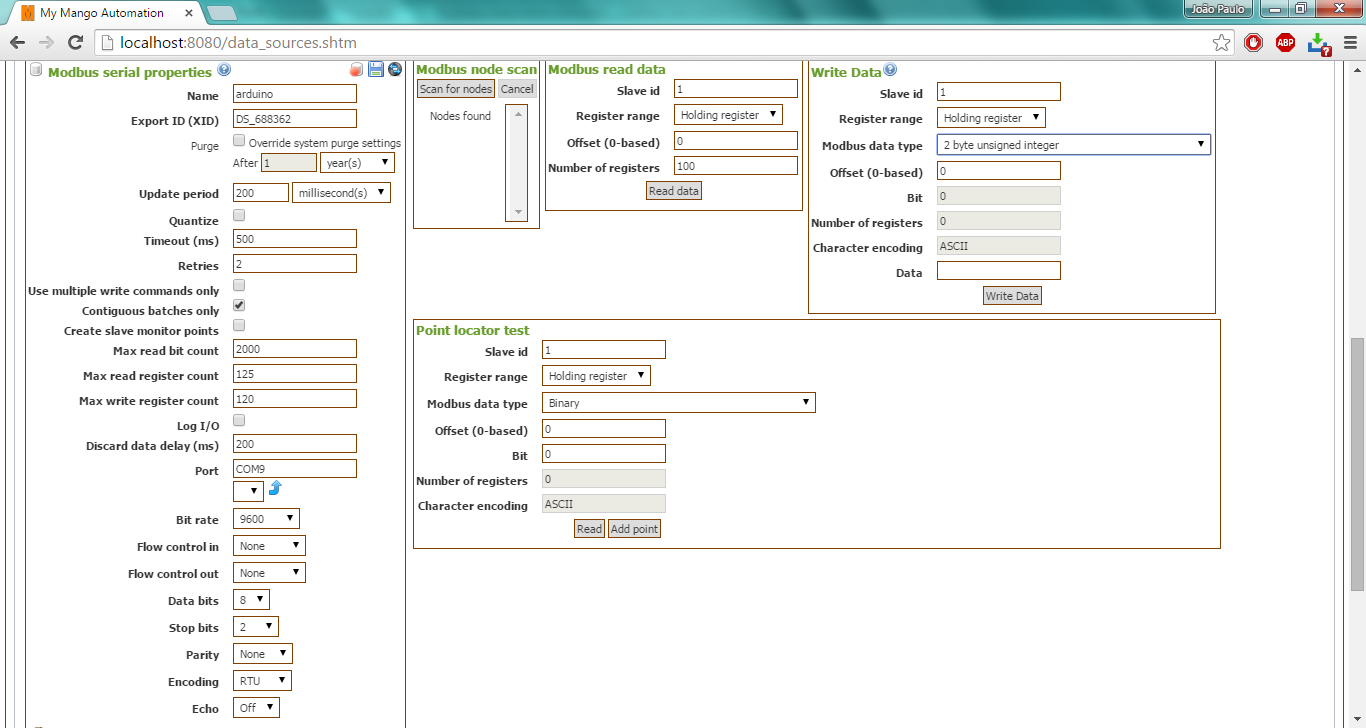
\includegraphics[width=\textwidth]{figuras/mango_modbus}
	\end{center}
	\caption{Definição de uma fonte de dados do tipo modbus serial.}
	\label{fig:mango_modbus}
\end{figure}

O modbus trabalha endereçando o escravo pelo \emph{slave id}, que no caso usamos 1. Os dados são armazenados nos chamados registradores (\emph{registers}). Enquanto o Modbus especifica 4 tipos de registradores, o arduino implementa apenas o \emph{Holding register}, logo nossos pontos devem ser todos deste tipo e concordar com a sequencia definida no arduino.
Cada registrador é de 16 bits. Podemos definir um ponto binário como sendo um único bit daquele registrador ou um ponto numérico, que usa todos os 16 bits.

\section{\emph{Watch list}}
Podemos observar o comportamento dos pontos criados na tela \emph{Watch lists} (figura \ref{fig:mango_watch}). Se o ponto for configurável (settable), também podemos fazé-lo por esta tela.

\begin{figure}[hbt]
	\begin{center}
		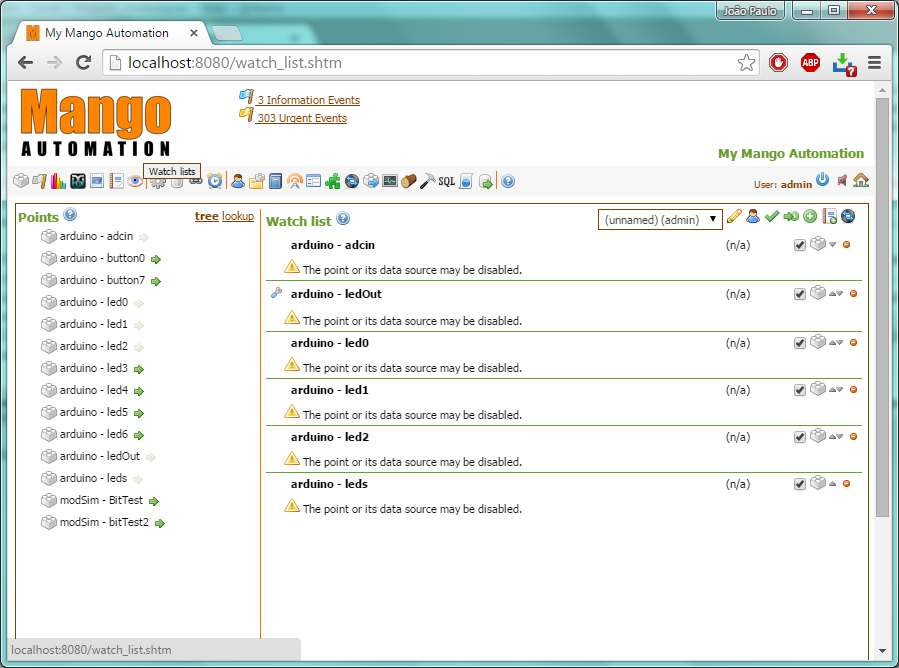
\includegraphics[width=\textwidth]{figuras/mango_watch}
	\end{center}
	\caption{\emph{Watch lists} para observar as variáveis.}
	\label{fig:mango_watch}
\end{figure}

\section{Tela gráfica}
A interface normal com o operador é feita através do sinótico -- a representação gráfica do processo. O mango permite montar uma tela gráfica apresentando os diversos valores das variáveis e os controles, como mostra a figura \ref{fig:mango_tela}. A apresentação de variáveis é de forma bem direta, através dos diversos comandos de gif analógico, gif binário, gif dinâmico e gráficos. O ajuste de valores, porém, é um pouco mais complexo.
\begin{figure}[hbt]
	\begin{center}
		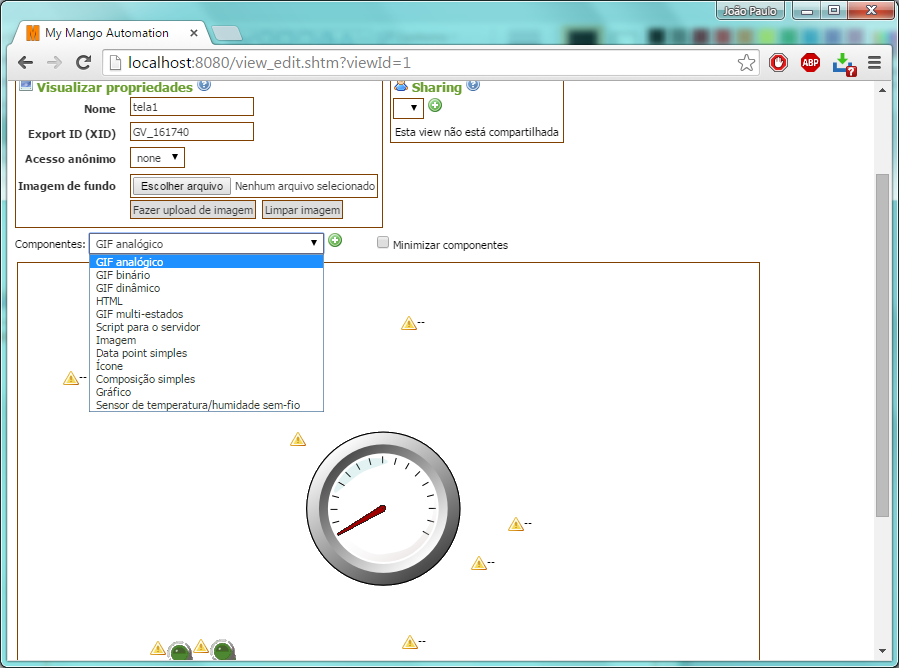
\includegraphics[width=\textwidth]{figuras/mango_tela}
	\end{center}
	\caption{Montagem de sinótico.}
	\label{fig:mango_tela}
\end{figure}

Pode-se ajustar o valor de um ponto no mango marcando a opção \textbf{Exibir controles}, a partir do que se pode abrir uma caixinha que permite a escrita do valor na variável. Esta opção porém é mutio pouco prática.

Outra opção mais interessante é através dos \emph{server side scripts}, ou scrpts do servidor. Nestes casos define-se um comando em javascript que permite ler e alterar o valor de uma variável. A página \textbf{http://infiniteautomation.com/wiki/doku.php?id=graphics:mango\_graphic\_views:server\_side\_script\_examples} mostra vários exemplos de códigos úteis para esta tarefa. 

Um adendo: os códigos da página supracitada consideram os endereços a partir da pasta \textbf{<mango>/web}. Porém o arquivo zipado do Mango não contém aí a subpasta Graphics, o que faz com que os exemplos não funcionem. é necessário copiar a pasta \textbf{<mango>/web/modules/sstGraphics/web/graphics} para este local. Pode-se (e deve-se) acrescentar outras imagens mais interessantes a este diretório.